\subtop{Menschliche Wahrnehmung}{-1.46}
\begin{description}
	\item[pre-attentive Vorverarbeitung]
	\item[Gestalt-Laws]\ \\\vspace*{-\baselineskip}
		\begin{itemize}
			\item Gesetz der Nachbarschaft (Proximity)
			\item Gesetz der Ähnlichkeit (Similarity)
			\item Gesetz der Verbundenheit (Connectedness)
			\item Gesetz der Fortführung (Continuity)
			\item Gesetz der Symmetrie
			\item Gesetz von Bild und Hintergund (Figure and Ground)
		\end{itemize}
	\item[Änderung der Blindheit] bei Fokusverlust gehen Veränderungen verloren
	\item[Genauigkeit der visuellen Variablen]\ \\\vspace*{-0.5\baselineskip}\\
		\usetikzlibrary{positioning}
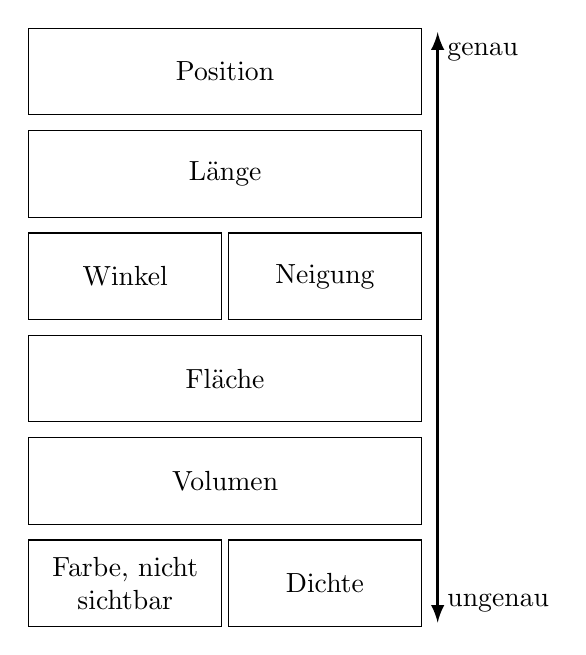
\begin{tikzpicture}[every node/.style={draw, minimum height=1.1cm, minimum width=5cm}]

	\node at(0,0) {Position};	
	\node at(0,-1.3) {L\"ange};
	\node[minimum width=2.45cm, anchor=west] at(-2.5,-2.6) {Winkel};
	\node[minimum width=2.45cm, anchor=east] at(2.5,-2.6) {Neigung};
	\node at(0,-3.9) {Fl\"ache};
	\node at(0,-5.2) {Volumen};
	\node[minimum width=2.45cm, anchor=west] at(-2.5,-6.5) {\begin{minipage}{2.2cm}\centering Farbe, nicht sichtbar\end{minipage}};
	\node[minimum width=2.45cm, anchor=east] at(2.5,-6.5) {Dichte};

\draw[<->, >=latex, very thick] (2.7,0.5) to (2.7,-7);
\node[draw=none, minimum width=0cm,minimum height=0cm, yshift=-0.25cm, anchor=west] at (2.7,0.5) {genau};
\node[draw=none, minimum width=0cm,minimum height=0cm, yshift=-0.25cm, anchor=west] at (2.7,-6.5) {ungenau};
\end{tikzpicture}
\end{description}